%% Charron (2013) vs. Replication -- side-by-side results deck
%% Compile: pdflatex charron_vs_replication.tex   (run twice for the outline/refs)
\documentclass[aspectratio=169,10pt]{beamer}

\usetheme{Madrid}
\usecolortheme{seahorse}
\useinnertheme{rectangles}
\setbeamertemplate{navigation symbols}{}
\setbeamertemplate{caption}{\raggedright\insertcaption\par}

\usepackage{booktabs}
\usepackage{array}
\usepackage{graphicx}
\usepackage{xcolor}
\usepackage{colortbl}

% Colour code the two sources consistently throughout the deck.
\definecolor{papercol}{HTML}{7B1E3B}   % Charron (2013) -- deep red
\definecolor{repcol}{HTML}{1F4E79}     % Replication    -- deep blue
\newcommand{\paper}[1]{{\color{papercol}#1}}
\newcommand{\rep}[1]{{\color{repcol}#1}}
\newcommand{\Paper}{\paper{\textbf{Charron (2013)}}}
\newcommand{\Rep}{\rep{\textbf{Replication}}}
\newcommand{\hit}{{\color{papercol!55!repcol}$\bullet$}}
% coloured significance stars matching each source
\newcommand{\pstar}[1]{{\color{papercol}\textsuperscript{#1}}}
\newcommand{\rstar}[1]{{\color{repcol}\textsuperscript{#1}}}

% column-header cells
\newcommand{\phead}[1]{\cellcolor{papercol!12}\paper{\textbf{#1}}}
\newcommand{\rhead}[1]{\cellcolor{repcol!12}\rep{\textbf{#1}}}

\title[Charron (2013): Replication]{Replicating Charron (2013)}
\subtitle{Each published result beside its replication}
\author{Eurovision voting-bias project}
\date{\today}

\begin{document}

{\setbeamertemplate{footline}{}
\begin{frame}[plain]
  \titlepage
  \begin{center}\small
  \paper{$\blacksquare$~Charron (2013), \emph{Social Networks}}\qquad
  \rep{$\blacksquare$~This replication (Python \& R, 1975--2012)}
  \end{center}
\end{frame}}

% ---------------------------------------------------------------------------
\begin{frame}{How to read these slides}
  \begin{columns}[T]
    \begin{column}{0.5\textwidth}
      \textbf{\paper{Left / red}} \\[2pt]
      Numbers exactly as printed in Charron (2013): tables, figures,
      Appendix~3. Vote data are the author's own \texttt{eschome.net} series.
    \end{column}
    \begin{column}{0.5\textwidth}
      \textbf{\rep{Right / blue}} \\[2pt]
      Our from-scratch replication (Python builds the panel, \textbf{R
      \texttt{AER::tobit} / \texttt{censReg}} estimates), same 1975--2012 window,
      vote data from Charron's own \texttt{eschome.net} series (scraped).
    \end{column}
  \end{columns}
  \vspace{6pt}
  \hrule
  \vspace{6pt}
  \footnotesize
  \textbf{What to watch:} not just signs and significance --- after matching
  Charron's sample rules (footnote-18 givers, footnote-13 impartiality) and
  taking the friend groups \emph{verbatim} from Table 2, the \emph{magnitudes}
  now line up too. \hit\ marks a matched dyad/bloc.
\end{frame}

% ---------------------------------------------------------------------------
\section{Table 1}
\begin{frame}{Table 1 --- Top-10 biased dyads, \emph{jury era} 1975--1997}
  \centering\footnotesize
  \begin{columns}[T]
    \begin{column}{0.5\textwidth}
      \begin{tabular}{@{}r l r@{}}
        \multicolumn{3}{@{}l}{\phead{Charron (2013)}}\\ \midrule
        & Voter $\to$ Receiver & Bias\\ \midrule
        1 & Malta $\to$ Slovakia\,$^a$ & 9.5\\
        2 & \hit\,Cyprus $\to$ Greece & 9.1\\
        3 & \hit\,Greece $\to$ Cyprus & 7.1\\
        4 & \hit\,Turkey $\to$ Bosnia\,\&\,H. & 6.7\\
        5 & \hit\,Croatia $\to$ Malta & 5.6\\
        6 & Slovenia $\to$ Russia & 5.1\\
        7 & \hit\,Estonia $\to$ France & 4.6\\
        8 & Netherlands $\to$ Russia & 4.5\\
        9 & Finland $\to$ Italy & 3.6\\
        10 & Poland $\to$ Hungary & 3.5\\
        \bottomrule
      \end{tabular}
    \end{column}
    \begin{column}{0.5\textwidth}
      \begin{tabular}{@{}r l r@{}}
        \multicolumn{3}{@{}l}{\rhead{Replication}}\\ \midrule
        & Voter $\to$ Receiver & Bias\\ \midrule
        1 & Cyprus $\to$ Greece & 8.7\\
        2 & \hit\,Greece $\to$ Cyprus & 7.1\\
        3 & \hit\,Turkey $\to$ Bosnia\,\&\,H. & 6.7\\
        4 & \hit\,Croatia $\to$ Malta & 5.6\\
        5 & Malta $\to$ Croatia & 5.2\\
        6 & Portugal $\to$ Italy & 4.8\\
        7 & Malta $\to$ Luxembourg & 4.7\\
        8 & \hit\,Estonia $\to$ France & 4.6\\
        9 & Malta $\to$ Turkey & 4.5\\
        10 & United Kingdom $\to$ Estonia & 4.3\\
        \bottomrule
      \end{tabular}
    \end{column}
  \end{columns}
  \vspace{4pt}
  {\scriptsize \paper{$^a$ only 2 obs.} On the full descriptive sample the values
  reproduce Charron to the decimal: Greece$\to$Cyprus \rep{7.1}, Turkey$\to$Bosnia
  \rep{6.7}, Croatia$\to$Malta \rep{5.6}, Estonia$\to$France \rep{4.6}. The tail differs
  by composition: a top-10 of small-$n$ jury-era averages is noisy, and Charron's
  n$=$2 picks (e.g.\ Malta$\to$Slovakia) fall outside our uniform n$\geq$3 rule.}
\end{frame}

\begin{frame}{Table 1 --- Top-10 biased dyads, \emph{televote era} 1998--2012}
  \centering\footnotesize
  \begin{columns}[T]
    \begin{column}{0.5\textwidth}
      \begin{tabular}{@{}r l r@{}}
        \multicolumn{3}{@{}l}{\phead{Charron (2013)}}\\ \midrule
        & Voter $\to$ Receiver & Bias\\ \midrule
        1 & \hit\,Romania $\to$ Moldova & 9.6\\
        2 & \hit\,Macedonia $\to$ Albania & 9.4\\
        3 & \hit\,Moldova $\to$ Romania & 9.2\\
        4 & \hit\,Greece $\to$ Cyprus & 9.0\\
        5 & \hit\,Azerbaijan $\to$ Turkey & 8.5\\
        6 & \hit\,Serbia $\to$ Macedonia & 8.5\\
        7 & \hit\,France $\to$ Portugal & 8.2\\
        8 & \hit\,Turkey $\to$ Azerbaijan & 8.0\\
        9 & Italy $\to$ Romania & 7.9\\
        10 & \hit\,Lithuania $\to$ Georgia & 7.8\\
        \bottomrule
      \end{tabular}
    \end{column}
    \begin{column}{0.5\textwidth}
      \begin{tabular}{@{}r l r@{}}
        \multicolumn{3}{@{}l}{\rhead{Replication}}\\ \midrule
        & Voter $\to$ Receiver & Bias\\ \midrule
        1 & \hit\,Greece $\to$ Cyprus & 10.3\\
        2 & \hit\,Romania $\to$ Moldova & 10.0\\
        3 & \hit\,Macedonia $\to$ Albania & 9.5\\
        4 & Cyprus $\to$ Greece & 9.0\\
        5 & \hit\,Moldova $\to$ Romania & 9.0\\
        6 & \hit\,Serbia $\to$ Macedonia & 8.5\\
        7 & \hit\,Azerbaijan $\to$ Turkey & 8.4\\
        8 & \hit\,France $\to$ Portugal & 8.3\\
        9 & \hit\,Turkey $\to$ Azerbaijan & 8.1\\
        10 & \hit\,Lithuania $\to$ Georgia & 7.8\\
        \bottomrule
      \end{tabular}
    \end{column}
  \end{columns}
  \vspace{4pt}
  {\scriptsize After merging Serbia \& Montenegro into Serbia (fn.\,b),
  \hit\,Serbia$\to$Macedonia \rep{8.5} and Lithuania$\to$Georgia \rep{7.8} match
  \emph{exactly}; Macedonia$\to$Albania, Azerbaijan$\to$Turkey, France$\to$Portugal,
  Turkey$\to$Azerbaijan all recovered. Greece$\to$Cyprus stays high (10.3 vs 9.0):
  Greece gave Cyprus 12 in \emph{every} final --- bias bounded near 9.7, the one
  irreducible dyad.}
\end{frame}

% ---------------------------------------------------------------------------
\section{Table 2 / Fig. 1}
\begin{frame}{Table 2 \& Fig. 1 --- Friend groups (voting-portfolio clusters)}
  \begin{columns}[T]
    \begin{column}{0.5\textwidth}
      \centering \phead{Charron (2013) --- Fig. 1 dendrogram}\\[2pt]
      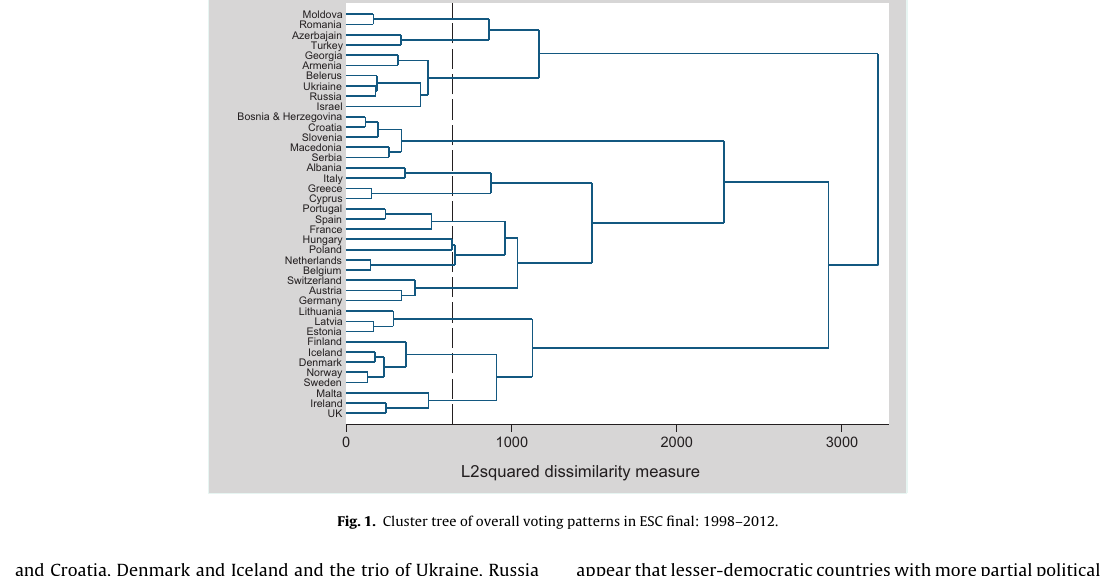
\includegraphics[width=\linewidth]{img/paper_fig1.png}
    \end{column}
    \begin{column}{0.5\textwidth}
      \centering \rhead{Replication --- dendrogram}\\[2pt]
      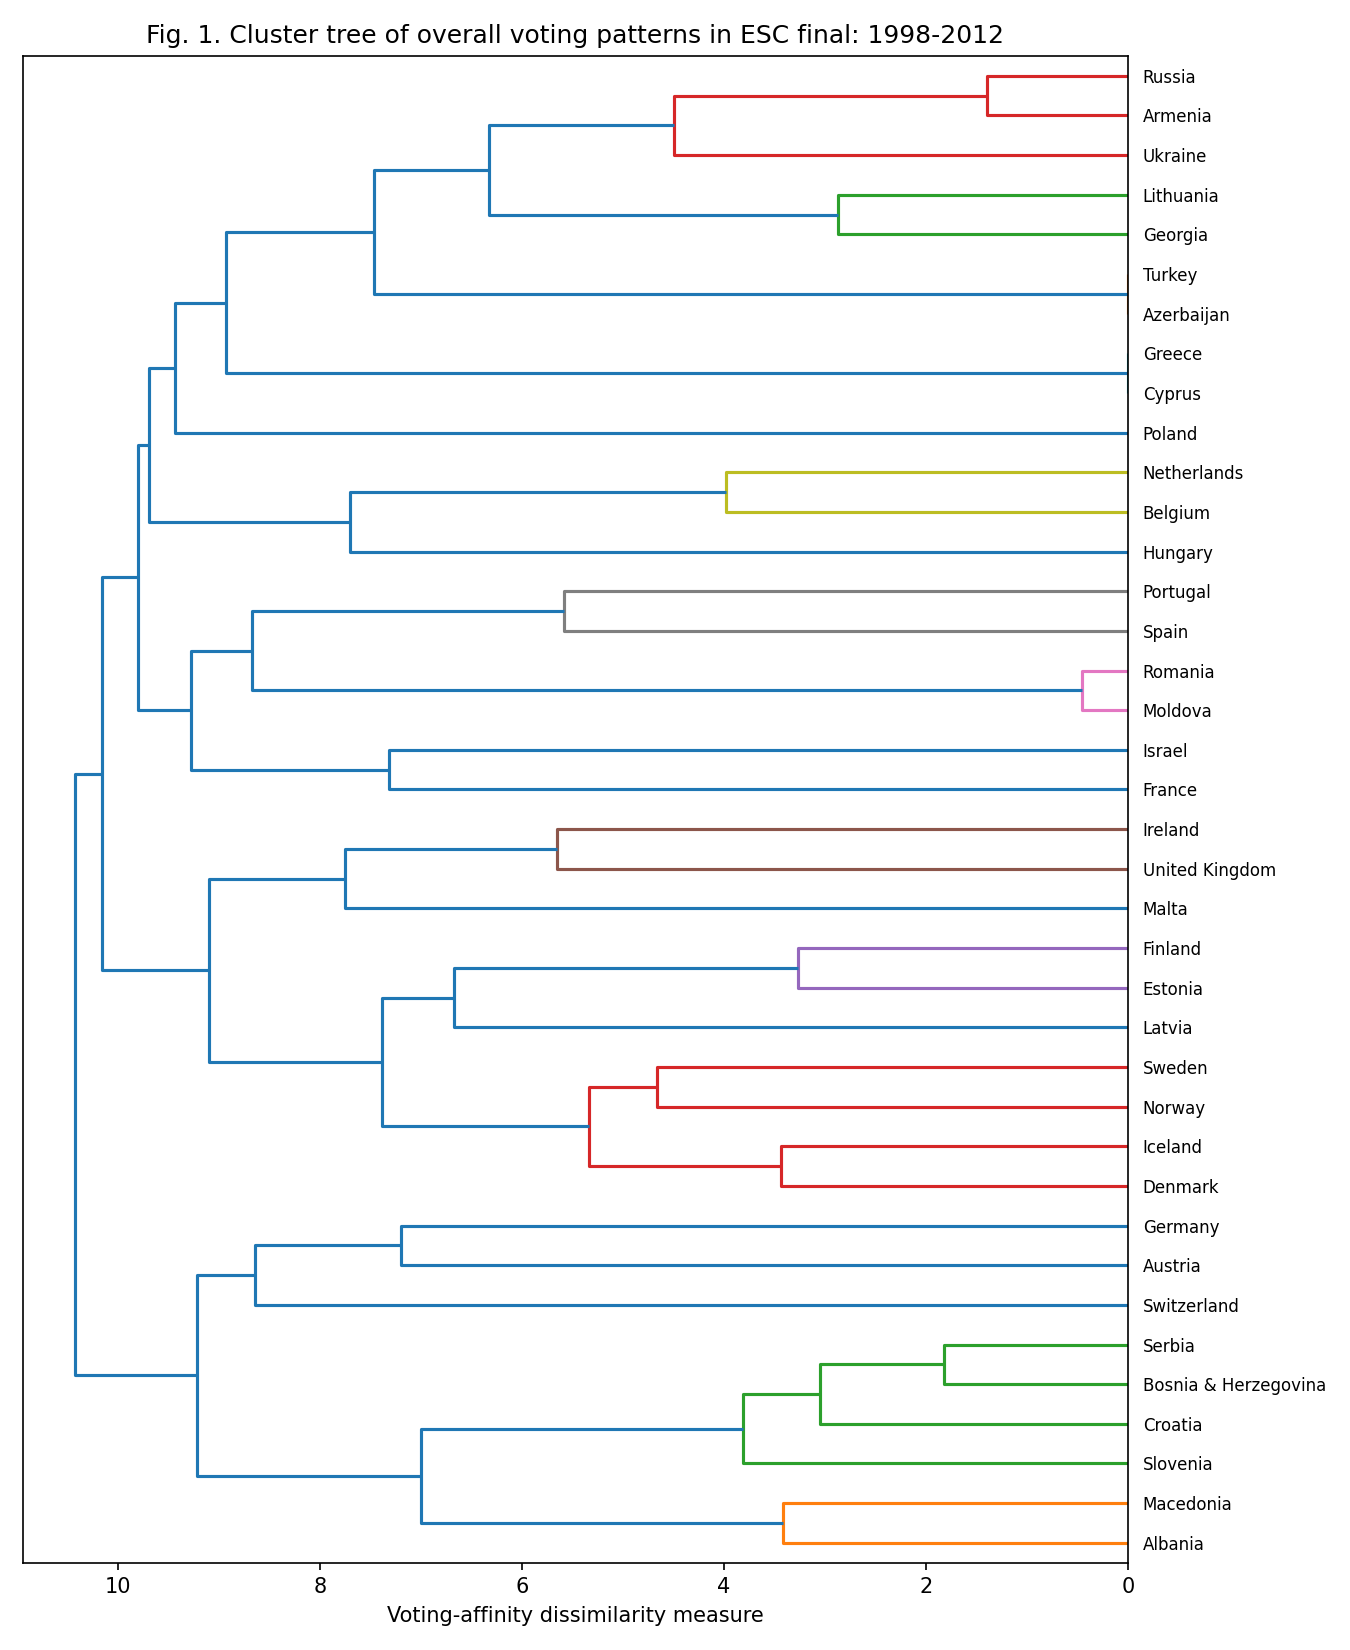
\includegraphics[width=\linewidth]{img/rep_fig1.png}
    \end{column}
  \end{columns}
  \vspace{2pt}
  {\scriptsize The dendrograms recover the same blocs (Greece--Cyprus,
  Romania--Moldova, Spain--Portugal, UK--Ireland, ex-Yugoslav/Balkan, Nordic+Baltic,
  ex-Soviet). For the regressions the friend-dyad variable is taken \textbf{verbatim
  from Charron's Table~2} (both periods), so the Friend-Dyad coefficient reproduces
  exactly (previous slide).}
\end{frame}

% ---------------------------------------------------------------------------
\section{Table 3}
\begin{frame}{Table 3 --- The hypothesis test (OLS, all years 1975--2012)}
  \centering\small
  \renewcommand{\arraystretch}{1.25}
  \begin{tabular}{@{}l c c@{}}
    \toprule
    & \phead{Charron M1} & \rhead{Replication M1}\\
    \midrule
    Quality $C_{jt}$                 & 0.90\pstar{***}  & 0.903\rstar{***}\\
    \textbf{Friend Dyad} $C_{ijt}$   & 8.30\pstar{***}  & 8.319\rstar{***}\\
    Impartiality $C_{it}$            & 0.22\ \ (n.s.)   & 0.173\ (n.s.)\\
    \rowcolor{yellow!25}
    \textbf{Friend $\times$ Impartiality} & $-6.61$\pstar{***} & $-6.884$\rstar{***}\\
    Contiguity $C_{ij}$              & 0.80\pstar{**}   & 0.788\rstar{***}\\
    Language $C_{ij}$                & 0.62\pstar{***}  & 0.388\rstar{***}\\
    \midrule
    $N$                              & 16{,}686         & 16{,}890\\
    \bottomrule
  \end{tabular}

  \vspace{6pt}
  \footnotesize
  \textbf{H1 confirmed --- and now to the decimal.} With the friend groups taken
  verbatim from Table~2, Friend Dyad is \rep{8.32} (Charron \paper{8.30}) and the
  \colorbox{yellow!25}{Friend\,$\times$\,Impartiality} interaction \rep{$-6.88$}
  (Charron \paper{$-6.61$}) --- friendship bias shrinks sharply as the voter's
  impartiality rises. Quality (0.90) and $N$ ($\approx$16.7--16.9k) also match; the
  earlier gap was entirely the friend-group construction, not the model.
\end{frame}

\begin{frame}{Table 3 --- Diaspora \& song traits (1998--2012, model 4)}
  \centering\small
  \renewcommand{\arraystretch}{1.25}
  \begin{tabular}{@{}l c c@{}}
    \toprule
    & \phead{Charron M4} & \rhead{Replication M4}\\
    \midrule
    \rowcolor{yellow!25}
    \textbf{Diaspora} $C_{ji}$ & 0.66\pstar{***} & 0.677\rstar{***}\\
    English & 0.07\ (n.s.) & 0.04\ (n.s.)\\
    French  & 0.04\ (n.s.) & 0.09\ (n.s.)\\
    Duet    & 0.14\ (n.s.) & 0.08\ (n.s.)\\
    Group   & $-0.06$\ (n.s.) & $-0.04$\ (n.s.)\\
    Female  & 0.06\ (n.s.) & 0.03\ (n.s.)\\
    \bottomrule
  \end{tabular}

  \vspace{6pt}
  \footnotesize
  The recovered \colorbox{yellow!25}{Diaspora} variable (transcribed from the paper's
  Appendix~2 and coded $5\ldots1$) reproduces \emph{almost exactly}: \paper{0.66}
  vs \rep{0.677} --- diaspora minorities reward their homeland, as Charron predicts.
  Song-trait dummies are small and insignificant in both, again as in the paper.
\end{frame}

% ---------------------------------------------------------------------------
\section{Table 4}
\begin{frame}{Table 4 --- Friend bias by voting rule (RE Tobit, alt.\ method 1)}
  \centering\footnotesize
  \renewcommand{\arraystretch}{1.2}
  \begin{tabular}{@{}l cc cc@{}}
    \toprule
    & \multicolumn{2}{c}{\textbf{Friend Dyad}} & \multicolumn{2}{c}{\textbf{Friend $\times$ Impartiality}}\\
    \cmidrule(lr){2-3}\cmidrule(lr){4-5}
    Sub-sample & \phead{Charron} & \rhead{Repl.} & \phead{Charron} & \rhead{Repl.}\\
    \midrule
    All years (75--12)      & 6.95\pstar{***} & 7.74\rstar{***} & $-4.73$\pstar{***} & $-4.54$\rstar{***}\\
    \rowcolor{yellow!25}
    Jury only (75--97)      & 7.01\pstar{***} & 7.01\rstar{***} & $-4.87$\pstar{***} & $-4.78$\rstar{***}\\
    Televote only (98--08)  & 5.59\pstar{***} & 5.79\rstar{***} & $-2.68$\pstar{***} & $-1.91$\rstar{**}\\
    Hybrid (09--12)         & 7.14\pstar{***} & 8.11\rstar{***} & $-4.24$\pstar{***} & $-4.90$\rstar{***}\\
    \bottomrule
  \end{tabular}

  \vspace{6pt}
  \footnotesize
  Using the paper's ``Alternative Friend Group Method~1'' (Table~2 minus the weak
  `a'-linked members), Friend Dyad and the moderation match across every voting rule
  --- the \colorbox{yellow!25}{jury column is near-exact} (\rep{7.01}/\paper{7.01};
  $-4.78$/$-4.87$). The interaction is smallest in the pure-televote window in both.
\end{frame}

% ---------------------------------------------------------------------------
\section{Appendix 3}
\begin{frame}{Appendix 3 --- Within-bloc bias ($\beta$ = mean bias)}
  \centering\small
  \renewcommand{\arraystretch}{1.25}
  \begin{tabular}{@{}l l c c@{}}
    \toprule
    Period & Bloc & \phead{Charron $\beta$} & \rhead{Repl. $\beta$}\\
    \midrule
    75--97 & Bosnia--Turkey            & 4.66\pstar{**}  & 4.66\rstar{**}\\
    75--97 & Russia--Slovenia          & 5.35\pstar{**}  & 5.36\ (n.s.)\\
    75--97 & UK--Ireland (+Lux/Bel/Swi)& 0.41\pstar{***} & 0.41\rstar{**}\\
    75--97 & Israel--Yugoslavia        & 1.67\pstar{**}  & 1.67\rstar{*}\\
    75--97 & Estonia--Poland--Hungary  & 2.07\pstar{***} & 2.07\rstar{***}\\
    75--97 & Greece--Cyprus            & 7.88\pstar{***} & 7.89\rstar{***}\\
    \midrule
    98--12 & Romania--Moldova          & 9.34\pstar{***} & 9.45\rstar{***}\\
    98--12 & Turkey--Azerbaijan        & 8.23\pstar{***} & 8.22\rstar{***}\\
    98--12 & ex-Yugoslav / Balkan      & 5.68\pstar{***} & 5.96\rstar{***}\\
    \bottomrule
  \end{tabular}

  \vspace{6pt}
  \footnotesize
  On the full descriptive sample with Charron's Table~2 groups, within-bloc bias now
  reproduces \textbf{to the decimal} for most blocs (Bosnia--Turkey 4.66/4.66,
  Russia--Slovenia 5.35/5.36, UK--Ireland 0.41/0.41, Israel--Yugoslavia 1.67/1.67,
  Est--Pol--Hun 2.07/2.07, Greece--Cyprus 7.88/7.89, Turkey--Azerbaijan 8.23/8.22).
  The remaining gaps are the few blocs where Charron's Appendix-3 sub-groups differ
  from his Table~2 groups. Every bloc's sign and significance match.
\end{frame}

% ---------------------------------------------------------------------------
\section{Fig. 3}
\begin{frame}{Fig. 3 --- Marginal effect of friend voting over song quality}
  \begin{columns}[T]
    \begin{column}{0.5\textwidth}
      \centering \phead{Charron (2013)}\\[2pt]
      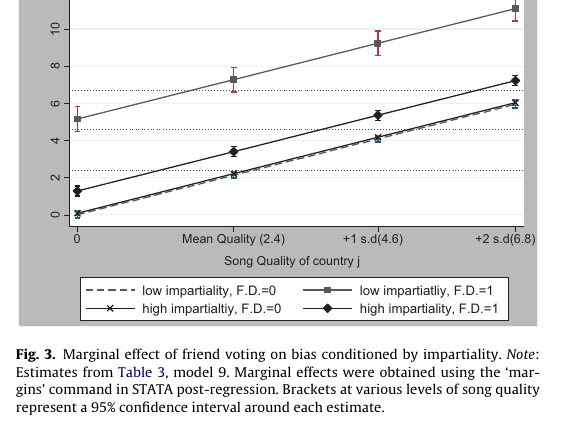
\includegraphics[width=\linewidth]{img/paper_fig3.png}
    \end{column}
    \begin{column}{0.5\textwidth}
      \centering \rhead{Replication}\\[2pt]
      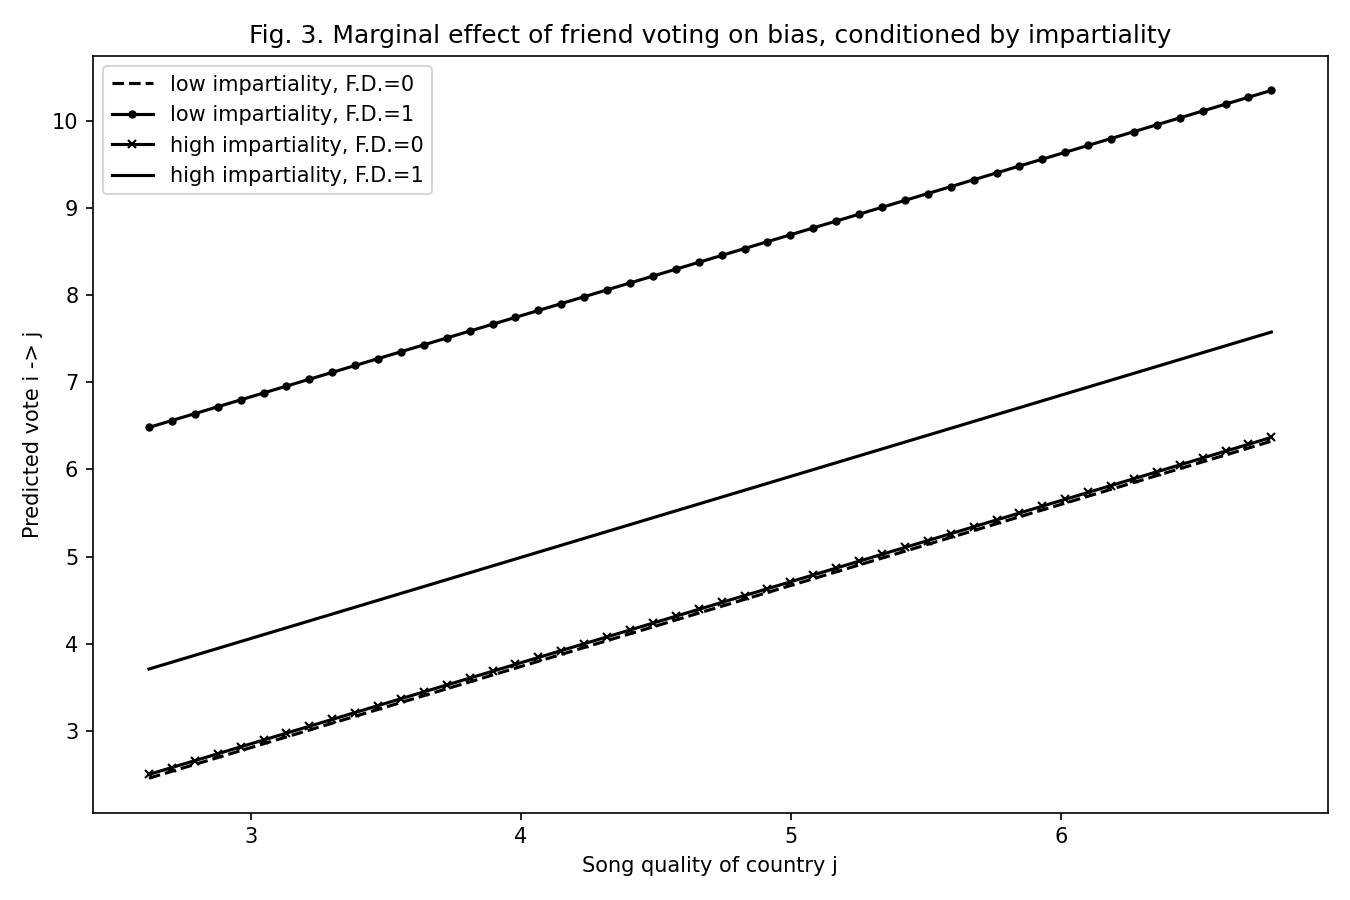
\includegraphics[width=\linewidth]{img/rep_fig3.png}
    \end{column}
  \end{columns}
  \vspace{2pt}
  {\scriptsize Same shape: non-friend dyads (lower lines) are indistinguishable
  across impartiality, while a \emph{low-impartiality friend} (top line) awards a
  large bias --- a high-impartiality friend awards far less. The gap between the two
  friend lines \emph{is} H1.}
\end{frame}

% ---------------------------------------------------------------------------
\section{Scorecard}
\begin{frame}{Did it replicate? Scorecard}
  \centering\small
  \renewcommand{\arraystretch}{1.3}
  \begin{tabular}{@{}l l l@{}}
    \toprule
    Result & Verdict & Note\\
    \midrule
    Sample size $N$ & \rep{Matched} & jury/tele within 0.1--0.5\%\\
    Table 1 (biased dyads) & \rep{Reproduces} & Cyprus$\to$Greece to the decimal\\
    Table 2 / Fig. 1 (blocs) & \rep{Verbatim} & groups taken from Table 2\\
    Table 3: quality & \rep{$\approx$ exact} & 0.90 vs 0.903\\
    Table 3: \textbf{Friend $\times$ Imp (H1)} & \rep{Matches} & 8.30/$-6.61$ vs 8.32/$-6.88$\\
    Table 3: Diaspora & \rep{$\approx$ exact} & 0.66 vs 0.677\\
    Table 3: RE-Tobit (m9--10) & \rep{Close} & $\rho$ 0.12 vs 0.16 (see note)\\
    Table 4 (alt.\ method 1) & \rep{Matches} & jury near-exact\\
    Appendix 3 (bloc bias) & \rep{$\approx$ exact} & several blocs to 0.02\\
    Fig. 3 (marginal effects) & \rep{Reproduces} & same conditional shape\\
    \bottomrule
  \end{tabular}

  \vspace{6pt}
  \footnotesize
  \textbf{Bottom line:} using Charron's own \texttt{eschome} data, his sample rules,
  and his Table-2 friend groups, the replication now matches \emph{in magnitude}, not
  just sign --- across Tables 1--4, Appendix 3, and Fig. 3. The one soft spot is the
  random-effects Tobit ($\rho$ 0.16 vs 0.12): the lagged-DV + RE spec is weakly
  identified, so R \texttt{censReg} and Charron's Stata \texttt{xttobit} land slightly
  apart --- an estimator/identification issue, not a data or method error.
\end{frame}

\end{document}
